\chapter{Generic simulation and problems of current hardware}

In the past year I have been researching protein folding and how to implement it on a general-purpose quantum computer. I have ran into a significant problem: I was unable to run any experiments of usable size, mainly due to limitations in memory. Due to quantum parallelism, the memory requirements of running a quantum calculation simulation are super-exponential. In particular, there is one component in Qiskit, which seemed to come back in any form of model I have tried to implement: a quantum gate for taking the sum of $n$ qubits, called the WeightedAdder class. 

This component came to my attention, because a natural way to encode protein structures is by creating a 2D or 3D grid and laying the aminoacid chain down on it\cite{dill_principles_2008}, as seen below.

\begin{figure}[H]
    \centering
    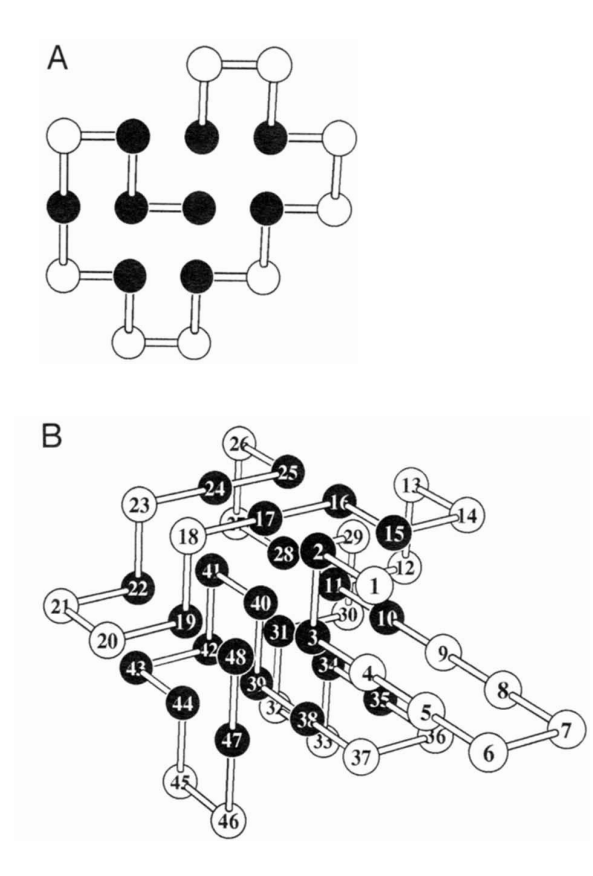
\includegraphics[width=0.5\linewidth]{figures/bioinformatics/hp_model.png}
    \caption{HP model of protein folding\cite{dill_principles_2008}}
\end{figure}

From a single vertex in a 3D grid, we can step in $4$ or $6$ directions: up, down, left, right and inwards and outwards in the 3D case. We can encode these naturally, using one-hot encoding, by introducing $6$ bits of information. If we assume that the chain starts in the origin, then we can encode a chain shape by giving the directions of the $(n-1)$ steps it takes.

A chain like this is viable, when it doesn't cross over itself. A chain's optimality is assessed by counting how many pairs of various aminoacids are neighbouring each other. To answer both of these questions, we must be able to calculate relative distances between any two points of the chain. Using the directinal one-hot encoding model, these questions can be answered by taking the sum of some qubits.

Using these operations, we can create a quantum oracle, that assesses the optimality of a particular chain and use Grover's quantum search algorithm to find the best possible solution.

Unfortunately, while Qiskit itself is open-source, it's architecture (similarly to other quantum computing frameworks) is designed from the core to store the matrices of various operations (such as the WeightedAdder operation) in its memory and retrieve this information during simulation. This means that I am unable to correct this single operation in Qiskit.